\documentclass[11pt]{article}
\usepackage{amsmath,amsthm,amssymb,fullpage,graphicx,hyperref}
\usepackage{listings,color,setspace}
\author{Andy Reagan}
\title{Math 337 Homework 15}

     \def\NN{\mathbb{N} }
     \def\ZZ{\mathbb{Z} }
     \def\QQ{\mathbb{Q} }
     \def\RR{\mathbb{R} }
     \def\CC{\mathbb{C} }
     \def\f{\frac }
     \def\b{\begin }
     \def\e{\end }
     \def\Log{\text{Log} \,}
     \def\Re{\text{Re} \, }
     \newcommand{\pdiff}[2]{\frac{\partial #1}{\partial #2}}
     \newcommand{\partialdiff}[2]{\frac{\partial #1}{\partial #2}}
     \newcommand{\pdiffsq}[2]{\frac{\partial^2 #1}{{\partial #2}^2}}
     \newcommand{\pdiffcu}[2]{\frac{\partial^3 #1}{{\partial #2}^3}}
     \newcommand{\pdiffhi}[3]{\frac{\partial^#3 #1}{{\partial #2}^#3}}
     \newcommand{\diff}[2]{\frac{{\rm d}#1}{{\rm d}#2}}
     \newcommand{\diffsq}[2]{\frac{{\rm d}^{2}#1}{{\rm d} {#2}^2}}
     \newcommand{\diffhi}[3]{\frac{{\rm d}^#3 #1}{{\rm d} {#2}^#3}}
     \newcommand{\tdiff}[2]{\mbox{d} #1/\mbox{d} #2}
     \newcommand{\tdiffsq}[2]{\mbox{d}^{2} #1/\mbox{d} {#2}^2}
     \newcommand{\tpdiff}[2]{\partial #1/\partial #2}
     \newcommand{\tpdiffsq}[2]{\partial^2 #1/\partial {#2}^2}
     \newcommand{\bvec}[1]{\vec{ {\bf #1 } }}
     \newcommand{\oh}[1]{O(h^{{#1}})}

\lstset{language=MATLAB,
basicstyle=\ttfamily\scriptsize\singlespacing,
keywordstyle=\color{black},
stringstyle=\color{black},
commentstyle=\color{black},
morecomment=[l][\color{black}]{\#},
frame=L,
xleftmargin=\parindent,
%%numbers=left,                   %% where to put the line-numbers
%%numberstyle=\scriptsize,      %% the size of the fonts that are used for the line-numbers
%%stepnumber=1,                   %% the step between two line-numbers. If it is 1 each line will be numbered
numbersep=5pt,
breaklines=true,        %% sets automatic line breaking
breakatwhitespace=false,    %% sets if automatic breaks should only happen at whitespace
escapeinside={\%*}{*)} 
}

%% example code insert
%% \lstinputlisting[language=Matlab]{andy_hw12_prb01.m}

%% example figure
%% \begin{figure}[h!]
%%   \centering
%%     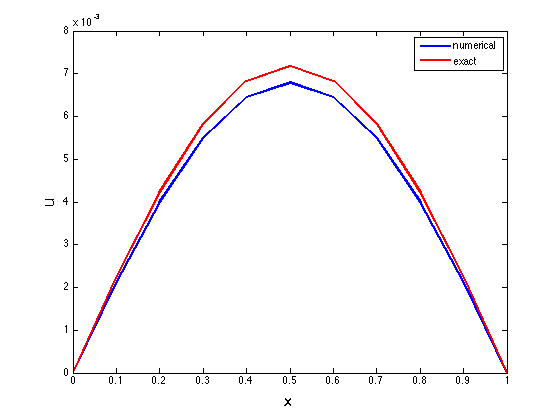
\includegraphics[width=0.45\textwidth]{andy_hw12_prb01_02.png}
%%   \caption{The numerical and exact solution for $h=0.1$.}
%% \end{figure}

%% start problem on next page
%% \clearpage
%% \pagebreak

\begin{document}
\maketitle

\begin{enumerate}

\item Code and a figure follow.

\lstinputlisting[language=Matlab]{andy_hw15_prb01.m}

\begin{figure}[h!]
  \centering
    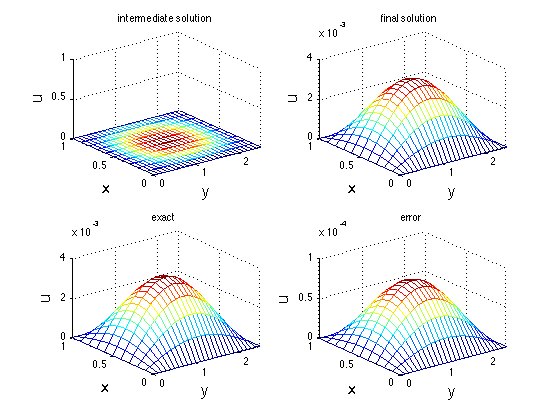
\includegraphics[width=0.8\textwidth]{andy_hw15_prb01_all.png}
    \caption{The intermediate solution, final solution, exact solution, and error for Problem 1 are plotted.}
\end{figure}

\item Code and a figure follow.

\lstinputlisting[language=Matlab]{andy_hw15_prb02.m}

\begin{figure}[h!]
  \centering
    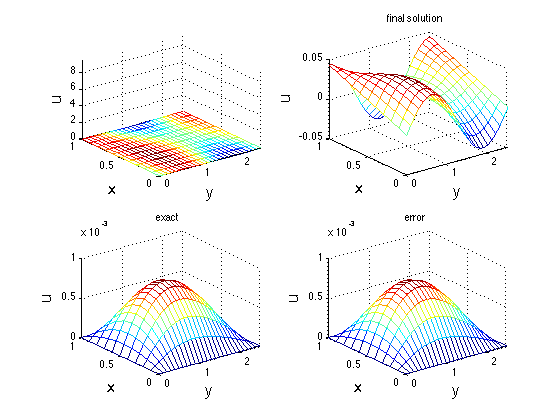
\includegraphics[width=0.8\textwidth]{andy_hw15_prb02_all.png}
    \caption{The intermediate solution, final solution, exact solution, and error for Problem 2 are plotted.}
\end{figure}

\item First we'll rewrite the half angle formula into a form more useful directly (starting the form given above Eq 12.35 in the notes):
\begin{align*} & 1-\cos \alpha = 2 \sin ^2 \left ( \f{\alpha}{2} \right ) \\
&2-2\cos \alpha = 4 \sin ^2 \left ( \f{\alpha}{2} \right ) \\
&2\cos \alpha - 2= - 4 \sin ^2 \left ( \f{\alpha}{2} \right ) \end{align*}
Now, we'll show Eq 15.12 directly.
\begin{align*} \delta _x ^2 \left [ e^{i\beta m h} e^{i\gamma l h} \right ] &= e^{i\beta (m+1) h} e^{i\gamma l h} -2 e^{i\beta m h} e^{i\gamma l h} + e^{i\beta (m-1) h} e^{i\gamma l h}\\
&= e^{i\beta m h} e^{i\gamma l h} \left [ e^{i\beta h}-2  + e^{-i\beta h} \right ]\\
&= e^{i\beta m h} e^{i\gamma l h} \left [ 2\cos (\beta h) -2 \right ]\\
&= e^{i\beta m h} e^{i\gamma l h} \left [ -4 \sin ^2 \left ( \f{\beta h}{2} \right ) \right ]\\
&= -4 \sin ^2 \left ( \f{\beta h}{2} \right )  \left [ e^{i\beta m h} e^{i\gamma l h}\right ]\end{align*}
We now do the same for Eq 15.13:
\begin{align*} \delta _y ^2 \left [ e^{i\beta m h} e^{i\gamma l h} \right ] &= e^{i\beta m h} e^{i\gamma (l+1) h} -2 e^{i\beta m h} e^{i\gamma l h} + e^{i\beta m h} e^{i\gamma (l-1) h}\\
&= e^{i\beta m h} e^{i\gamma l h} \left [ e^{i\gamma h}-2  + e^{-i\gamma h} \right ]\\
&= e^{i\beta m h} e^{i\gamma l h} \left [ 2\cos (\gamma h) -2 \right ]\\
&= e^{i\beta m h} e^{i\gamma l h} \left [ -4 \sin ^2 \left ( \f{\gamma h}{2} \right ) \right ]\\
&= -4 \sin ^2 \left ( \f{\gamma h}{2} \right )  \left [ e^{i\beta m h} e^{i\gamma l h}\right ]\end{align*}

% 4
\item We have the PDE
\[ u_t = a \left ( u_{xx} + u_{yy} \right ) + f(x,y,t). \]
We start by rewriting equation (15.16) for this PDE, and we have
\[ \vec{U} _{ml} ^{n+1} = \vec{U} _{ml} ^{n} + \f{ar}{2} \left ( \delta _x ^2 + \delta _y ^2 \right )  \left ( \vec{U} _{ml} ^{n} + \vec{U} _{ml} ^{n+1} \right ) + \f{\kappa}{2} \left ( f(x_m,y_l,t_n ) + f(x_m,y_l,t_{n+1}  ) \right ) .\]
From here, we can write down the generalization of Eq (15.24):
\[ \left ( \mathcal{I} + a\mathcal{A} \right) \vec{U} ^{n+1}  = \left ( \mathcal{I} - a\mathcal{A} \right) \vec{U} ^n + \f{\kappa}{2} \left ( f(\vec{x},\vec{y},t_n ) + f(\vec{x}, \vec{y},t_{n+1}  ) \right ) \]
where we will have ordered $f$ into a vector using the same ordering as we did for $\vec{U}^n$ and $\vec{U}^{n+1}$

% 5
\item We have the Douglas method:
\begin{align*} (a) &: ~~~~ \left ( 1 - \f{r}{2}\delta _x ^2 \right ) U^* _{ml} = \left ( 1  + \f{r}{2} \delta _x ^2 + r \delta _y ^2 \right ) U^n _{ml} \\
(b) &: ~~~~ \left ( 1 - \f{r}{2}\delta _y ^2  \right ) U^{n+1}  _{ml} = U^* _{ml} - \f{r}{2} \delta _y ^2 U^n _{ml} \end{align*} 
Multiplying Eq (b) by $\left ( 1 - \f{r}{2}\delta _x ^2 \right )$, we have
\[ \left ( 1 - \f{r}{2}\delta _x ^2 \right ) \left ( 1 - \f{r}{2}\delta _y ^2  \right ) U^{n+1}  _{ml} = \left ( 1 - \f{r}{2}\delta _x ^2 \right )U^* _{ml} - \left ( \f{r}{2} \delta _y ^2 - \left ( \f{r}{2} \right ) ^ 2 \delta _x ^2 \delta _y ^2\right ) U^n _{ml} \]
Plugging in the RHS of Eq (a) of the Douglas method for the $\left ( 1 - \f{r}{2}\delta _x ^2 \right ) U^* _{ml}$ term, we have
\begin{align*}  \left ( 1 - \f{r}{2}\delta _x ^2 \right ) \left ( 1 - \f{r}{2}\delta _y ^2  \right ) U^{n+1}  _{ml} &= \left ( 1  + \f{r}{2} \delta _x ^2 + r \delta _y ^2 \right ) U^n _{ml} - \left ( \f{r}{2} \delta _y ^2 - \left ( \f{r}{2} \right ) ^ 2 \delta _x ^2 \delta _y ^2\right ) U^n _{ml} \\
&= \left ( 1  + \f{r}{2} \delta _x ^2 + r \delta _y ^2  - \f{r}{2} \delta _y ^2 + \left ( \f{r}{2} \right ) ^ 2 \delta _x ^2 \delta _y ^2\right ) U^n _{ml} \\
&= \left ( 1  + \f{r}{2} \delta _x ^2 + \f{r}{2} \delta _y ^2 + \left ( \f{r}{2} \right ) ^ 2 \delta _x ^2 \delta _y ^2\right ) U^n _{ml} \\
&= \left ( 1  + \f{r}{2} \delta _x ^2  \right ) \left ( 1 + \f{r}{2} \delta _y ^2 \right ) U^n _{ml} \end{align*}
which is the same as Eq (15.33), as desired.

Now, we verify the stability condition found in the notes.
First, we plug (15.40) into (15.48), and we have
\begin{align*} (a) &: ~~~~ \left ( 1 - \f{r}{2}\delta _x ^2 \right ) \rho ^n \rho ^* e^{i\beta m h } e^{ i \gamma l h} = \left ( 1  + \f{r}{2} \delta _x ^2 + r \delta _y ^2 \right ) \rho^n e^{i\beta m h } e^{ i \gamma l h}\\
(b) &: ~~~~ \left ( 1 - \f{r}{2}\delta _y ^2  \right ) \rho^{n+1}  e^{i\beta m h } e^{ i \gamma l h} = \rho^n \rho ^* e^{i\beta m h } e^{ i \gamma l h} - \f{r}{2} \delta _y ^2 \rho ^n e^{i\beta m h } e^{ i \gamma l h} \end{align*} 
Using Eq (15.12,15.13), we apply the $\delta$ operators, and cancel the common $\rho ^n e^{i\beta m h } e^{ i \gamma l h}$:
\begin{align*} (a) &: ~~~~ \left ( 1 - \f{1}{2} \left [ -4r \sin ^2 \left (\f{\beta h}{2} \right ) \right ] \right ) \rho ^* = 1  + \f{1}{2} \left [ -4r \sin ^2 \left (\f{\beta h}{2} \right ) \right ] + \left [ -4r \sin ^2 \left (\f{\gamma h}{2} \right ) \right ] \\
(b) &: ~~~~ \left ( 1 - \left [ -4r \sin ^2 \left (\f{\gamma h}{2} \right ) \right ] \right ) \rho = \rho ^* - \f{1}{2} \left [ -4r \sin ^2 \left (\f{\gamma h}{2} \right ) \right ] \end{align*} 
Using the shorthand $X = 2r \sin ^2 \left (\f{\beta h}{2} \right )$ and $Y = 2r \sin ^2 \left (\f{\gamma h}{2} \right )$, we write as
\begin{align*} (a) &: ~~~~ \left ( 1 + X \right ) \rho ^* = \left ( 1 - X - 2Y \right )  \\
(b) &: ~~~~ \left ( 1 + Y \right  ) \rho = \rho ^* + Y \end{align*} 
Equation (a) simplifies to
\[ \rho ^* = \f{1-X-2Y}{1+X} \]
and Equation (b) then becomes
\[ \rho = \f{\rho ^* + Y}{1+Y} = \f{\f{1-X-2Y}{1+X} + Y}{1+Y} = \f{\f{1-X-2Y+Y+YX}{1+X}}{1+Y} = \f{1-X-Y+YX}{(1+X)(1+Y)} = \f{(1-X)(1-Y)}{(1+X)(1+Y)}, \]
as desired.

% 6
\item First I make note of the very important considerations mentioned in the paragraph following Eq 15.37, which make clear the notation that we are using.
Namely, we are solving for a solution in a 2D space (with solution represented as a matrix), where discretizations have been made in orthogonal directions.
We choose to break this into a smaller problems: we solve not for the full solution at the next timestep, but rather we solve for each column, one at a time.
In doing so, we first break the problem in columns, which in turn determines which operators act as matrices on a columns, and which operate across columns.
We have chosen to break into columns where $m$ varies, namely columns for each $l$.
Doing this, we arrive at Eq 15.37.
To make this more clear, consider Eq 15.37 in matrix form:
\begin{align*} & \left [ \left ( \begin{array}{ccc} 1 & 0 & 0\\ 0 & 1 & 0\\ 0 & 0 & 1 \end{array} \right )  - \f{r}{2} \left ( \begin{array}{ccc} -2 & 1 & 0\\ 1 & -2 & 1\\ 0 & 1 & -2 \end{array} \right )\right ] \left ( \begin{array}{c} U_{1,l} \\ U_{2,l} \\ U_{3,l} \end{array} \right ) ^{*} = \left ( \begin{array}{c} U_{1,l} \\ U_{2,l} \\ U_{3,l} \end{array} \right ) ^{n} \\
&~~~~~~~~~~~~~~~+ \f{r}{2} \left [ \left ( \begin{array}{c} U_{1,l+1} \\ U_{2,l+1} \\ U_{3,l+1} \end{array} \right ) ^{n} - 2\left ( \begin{array}{c} U_{1,l} \\ U_{2,l} \\ U_{3,l} \end{array} \right ) ^{n} + \left ( \begin{array}{c} U_{1,l-1} \\ U_{2,l-1} \\ U_{3,l-1} \end{array} \right ) ^{n}\right ] \end{align*}
Since $L = 5$, we solve for $U^{*}$ for $l = 1\cdot 4$, where the BC of $U^{*}$ at $l = 0, 5$ are given by the prescribed conditions.
Here, they are just 0.
We observe that for $l=1$ and $l=4$ the RHS $U^{n}$ will have $l=0,5$ respectively, where here we invoke the BC.
So what we are really solving for is a $(M-2) \times (L-2)$ matrix from a $M\times L$ matrix, solving for only the inner points.

We could write out the previous equation for each $L$, but this is cumbersome and is not how we will solve the problem on a computer.
Namely, we will solve this as a matrix, for all of the columns.
Without further adieu, this is:
\begin{align*} & \left [ \left ( \begin{array}{ccc} 1 & 0 & 0\\ 0 & 1 & 0\\ 0 & 0 & 1 \end{array} \right )  - \f{r}{2} \left ( \begin{array}{ccc} -2 & 1 & 0\\ 1 & -2 & 1\\ 0 & 1 & -2 \end{array} \right )\right ] \left ( \begin{array}{cccc} U_{1,1} & U_{1,2} & U_{1,3} & U_{1,4 }\\ U_{2,1} & U_{2,2} & U_{2,3} & U_{2,4 } \\ U_{3,1} & U_{3,2} & U_{3,3} & U_{3,4 }  \end{array} \right ) ^{*} \\
& ~~~~~~~~~= \left ( \begin{array}{cccc} U_{1,1} & U_{1,2} & U_{1,3} & U_{1,4 }\\ U_{2,1} & U_{2,2} & U_{2,3} & U_{2,4 } \\ U_{3,1} & U_{3,2} & U_{3,3} & U_{3,4 }  \end{array} \right ) ^{n} + \f{r}{2} \left [ \left ( \begin{array}{cccc} U_{1,2} & U_{1,3} & U_{1,4} & 0 \\ U_{2,2} & U_{2,3} & U_{2,4} & 0 \\ U_{3,2} & U_{3,2} & U_{3,4} & 0  \end{array} \right ) ^{n} \right.\\
& ~~~~~~~~~\left. -2\left ( \begin{array}{cccc} U_{1,1} & U_{1,2} & U_{1,3} & U_{1,4 }\\ U_{2,1} & U_{2,2} & U_{2,3} & U_{2,4 } \\ U_{3,1} & U_{3,2} & U_{3,3} & U_{3,4 }  \end{array} \right ) ^{n} + \left ( \begin{array}{cccc} 0 & U_{1,1} & U_{1,2} & U_{1,3 }\\ 0 & U_{2,1} & U_{2,2} & U_{2,3 } \\ 0 & U_{3,1} & U_{3,2} & U_{3,3 }  \end{array} \right ) ^{n} \right ]\end{align*}

Regardless about solving on the computer, from the above is obvious how the problem is split into columns.
If it is not, just take the first column from every $3\times 4$ matrix for the first column problem, the second column from every $3\times 4$ matrix for the second column problem, and so forth.
The boundary conditions have entered visibly only in $l$ since they are zero.
If they were nonzero along $x=0$ or $x=M$ the $3\times 3$ matrix on the LHS (resulting from the addition) would need a $\bvec{b}$ vector on the LHS when solving for each column, added outside what is already there, with the nonzero boundary conditions included at the beginning and end of this vector as we have done in the past.
In the matrix form above, this would actually be a matrix, $\bvec{B}$.

Next, we write Eq 15.34(b) 
\begin{align*} & \left [ \left ( \begin{array}{cccc} 1 & 0 & 0 & 0\\ 0 & 1 & 0 & 0\\ 0 & 0 & 1 & 0\\ 0 & 0 & 0 & 1\end{array} \right )  - \f{r}{2} \left ( \begin{array}{cccc} -2 & 1 & 0 & 0 \\ 1 & -2 & 1 & 0\\ 0 & 1 & -2 & 1\\ 0 & 0 & 1 & -2\end{array} \right )\right ] \left ( \left ( \begin{array}{cccc} U_{1,1} & U_{1,2} & U_{1,3} & U_{1,4 }\\ U_{2,1} & U_{2,2} & U_{2,3} & U_{2,4 } \\ U_{3,1} & U_{3,2} & U_{3,3} & U_{3,4 }  \end{array} \right ) ^T \right ) ^{n+1} \\
& ~~~~~~~~~= \left ( \left ( \begin{array}{cccc} U_{1,1} & U_{1,2} & U_{1,3} & U_{1,4 }\\ U_{2,1} & U_{2,2} & U_{2,3} & U_{2,4 } \\ U_{3,1} & U_{3,2} & U_{3,3} & U_{3,4 }  \end{array} \right )  ^T \right )  ^{*} + \f{r}{2} \left [ \left ( \left ( \begin{array}{cccc} U_{1,2} & U_{1,3} & U_{1,4} & 0 \\ U_{2,2} & U_{2,3} & U_{2,4} & 0 \\ U_{3,2} & U_{3,2} & U_{3,4} & 0  \end{array} \right ) ^T \right ) ^{*} \right.\\
& ~~~~~~~~~\left. -2\left ( \left ( \begin{array}{cccc} U_{1,1} & U_{1,2} & U_{1,3} & U_{1,4 }\\ U_{2,1} & U_{2,2} & U_{2,3} & U_{2,4 } \\ U_{3,1} & U_{3,2} & U_{3,3} & U_{3,4 }  \end{array} \right ) ^T \right ) ^{*} + \left ( \left ( \begin{array}{cccc} 0 & U_{1,1} & U_{1,2} & U_{1,3 }\\ 0 & U_{2,1} & U_{2,2} & U_{2,3 } \\ 0 & U_{3,1} & U_{3,2} & U_{3,3 }  \end{array} \right ) ^T \right ) ^{*} \right ]\end{align*}

where again we can solve this equation column by column for the three columns of $U^{n+1}$ in matrix form above.

% 7
\item This was already discussed in problem 6, in a manner in which is sufficient to code.
But I will still elaborate more.
Specifically, we first solve for $U ^*$ column by column, and the using this $U^*$, we solve for $U ^{n+1}$ column by column.
This is:
\begin{itemize}
\item Set the boundaries of $U^*$ using the boundaries of both $U^{n}$ and $U^{n+1}$, which we know from the BC
\item Solve for the interior of $U^*$ from $U^{n}$ and the BC of $U^*$ that we now have.
\item Set the boundaries of $U^{n+1}$ using the BC.
\item Solve for the interior of $U^{n+1}$ from $U^{*}$ and the BC of $U^{n+1}$ that we have set.
\end{itemize} 

I am inclined to try solving this as a matrix eqaution, as we discussed in class, and if I try this to compare, I will report on the results.
Of course, this is only reasonable to try for the case of 0 boundary conditions, since even for Dirichlet BC the determination of the BC of the intermediate solution $U^*$ is no longer trivial.
Pre-computing $\bvec{b}^*$ could, in theory, make this possible even for nonzero BC conditions.

I'll note that I choose to update the BC for $U^{n+1}$ just before I solve for the interior of $U^{n+1}$, since this makes the most sense to me (determing $U^{n+1}$ happens in one place).

% 8
\item I solve the problem using the method that was exhaustively elaborated upond above.

I am able to solve the problem as a matrix, and gain a huge speedup by doing so.
It is important to clear the namespace before testing the speed.
I have included a script which does this comparison 100 times, and averages the result.

When I ran this script, I got an average speedup of $9.92 \times$ over 100 trials.
The script is included after the code to solve this problem.

\lstinputlisting[language=Matlab]{andy_hw15_prb08.m}

\lstinputlisting[language=Matlab]{andy_hw15_prb08_matrix.m}

\lstinputlisting[language=Matlab]{andy_hw15_prb08_noplots.m}

\lstinputlisting[language=Matlab]{andy_hw15_prb08_compare.m}

\begin{figure}[h!]
  \centering
    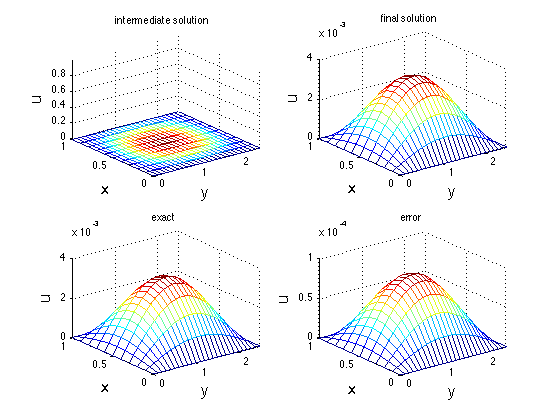
\includegraphics[width=0.8\textwidth]{andy_hw15_prb08_all.png}
    \caption{The intermediate solution, final solution, exact solution, and error for Problem 8 are plotted.}
\end{figure}

% 9
\item The boundary conditions are not difficult to implement in this case, and I solve the problem in the following code:

\lstinputlisting[language=Matlab]{andy_hw15_prb09.m}

\begin{figure}[h!]
  \centering
    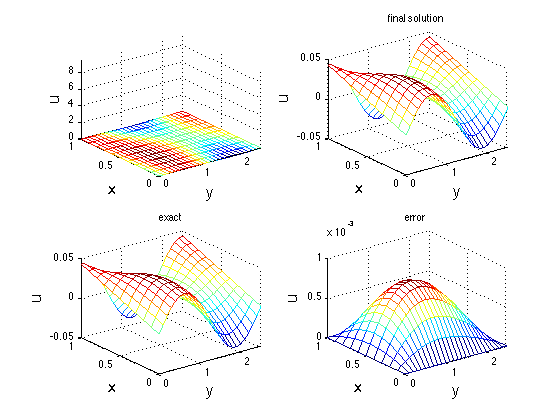
\includegraphics[width=0.8\textwidth]{andy_hw15_prb09_all.png}
    \caption{The intermediate solution, final solution, exact solution, and error for Problem 9 are plotted.}
\end{figure}

% 10 
\item For the Douglas method, which is
\begin{align*} (a) &: ~~~~ \left ( 1 - \f{r}{2}\delta _x ^2 \right ) U^* _{ml} = \left ( 1  + \f{r}{2} \delta _x ^2 + r \delta _y ^2 \right ) U^n _{ml} \\
(b) &: ~~~~ \left ( 1 - \f{r}{2}\delta _y ^2  \right ) U^{n+1}  _{ml} = U^* _{ml} - \f{r}{2} \delta _y ^2 U^n _{ml}, \end{align*} 
in Eq (a) we have the whole mesh on the RHS for $U^n$, and for the LHS we are discretized along $x$ so we will need the $x$ boundaries at $0,M$ in $U^*$.
Looking at Eq (b), knowing that we need the $x=0,M$ boundaries of $U^*$, we observe that we can solve for these in Eq (b).
Namely, we write (b) as
\[ \left ( 1 - \f{r}{2}\delta _y ^2  \right ) U^{n+1}  _{0l} = U^* _{0l} - \f{r}{2} \delta _y ^2 U^n _{0l}, \]
and since we already know $U^{n+1}  _{0l}$ and $U^{n}  _{0l}$, we can solve for $U^* _{0l}$ as
\[  U^* _{0l} = \f{r}{2} \delta _y ^2 U^n _{0l} + \left ( 1 - \f{r}{2}\delta _y ^2  \right ) U^{n+1}  _{0l} \]
and
\[  U^* _{Ml} = \f{r}{2} \delta _y ^2 U^n _{Ml} + \left ( 1 - \f{r}{2}\delta _y ^2  \right ) U^{n+1}  _{Ml}. \]
This agrees with the notes, Eq (15.74).

Now for the D'yaknonov method,
\begin{align*} (a) &: ~~~~ \left ( 1 - \f{r}{2}\delta _x ^2 \right ) U^* _{ml} = \left ( 1  + \f{r}{2} \delta _x ^2 \right ) \left ( 1 + r \delta _y ^2 \right ) U^n _{ml} \\
(b) &: ~~~~ \left ( 1 - \f{r}{2}\delta _y ^2  \right ) U^{n+1}  _{ml} = U^* _{ml}, \end{align*} 
and in (a) we need all of $U^n$ on the RHS to solve for the interior of $U^*$ on the LHS.
Also, since the discretization is in $x$ on the LHS, we will also need the $x=0,M$ boundaries of $U^*$ to solve for $U^*$ on the interior.
In Eq (b) we only need the interior of $U^*$ on the RHS to solve for the interior of $U^{n+1}$, and need all of $U^{n+1}$ on the LHS, which we have from the BC.
Therefore, we solve for the $x=0,M$ boundaries in Eq (b) using the known boundaries of $U^{n+1}$, and this amount to solve (b) at $x=0,M$ for $U^*$ which is
\[ U^* _{0l} = \left ( 1 - \f{r}{2}\delta _y ^2  \right ) U^{n+1}  _{0l} \]
and 
\[ U^* _{Ml} = \left ( 1 - \f{r}{2}\delta _y ^2  \right ) U^{n+1}  _{Ml} \]

Finally, we consider the 3 dimensional extension of the Douglas Method.
The method is:
\begin{align*} (a) &: ~~~~ \left ( 1 - \f{r}{2}\delta _x ^2 \right ) U^* _{mlj} = \left ( 1  + \f{r}{2} \delta _x ^2 + r \delta _y ^2 + r \delta _z ^2 \right ) U^n _{mlj} \\
(b) &: ~~~~ \left ( 1 - \f{r}{2}\delta _y ^2  \right ) U^{**}  _{mlj} = U^* _{mlj} - \f{r}{2} \delta _y ^2 U^n _{mlj}, \\
(c) &: ~~~~ \left ( 1 - \f{r}{2}\delta _z ^2  \right ) U^{n+1}  _{mlj} = U^{**} _{mlj} - \f{r}{2} \delta _z ^2 U^n _{mlj}. \end{align*} 
I'll explain what we need, and what we have, for each side of each equation in words.
Then I'll explain how we'll get them.

In (a), on the RHS we eed $U^n$ at all boundaries, and we have this.
On the LHS we need $U^*$ at the $x=0,M$ boundaries since the discretization is in $x$.

In (b), on the RHS we need $U^n$ at the $y$ boundary, and we have this.
We also need $U^*$ on the interior, and we will presume to have this from (a).
On the LHS we need $U^{**}$ at the $y=0,L$ boundaries since the discretization is in $y$.

Finally, in (c), on the RHS we need $U^n$ at the $z$ boundary, and we have this.
We also need $U^{**}$ on the interior, and we will presume to have this from (b).
On the LHS we need $U^{n+1}$ at the $z=0,K$ boundaries since the discretization is in $z$.

Given all of this discussion, it is now clear how we will solve for each these.
In short, we will solve for $U^{**}$ at the $x$ and $y$ boundaries from (c), and then solve for $U^*$ at the $x$ boundary from (b).
We could go about showing how we arrive at the aforementioned solution by solving (b) for the $x$ boundaries in $U^*$, since this is only place that we {\em could} get them.
Then we will have needed $U^{**}$ at the $x$ and $y$ boundaries, which we solve for in (c).
So we first solve for the $x$ boundaries of $U^{**}$ in (c):
\[ \left ( 1 - \f{r}{2}\delta _z ^2  \right ) U^{n+1}  _{0lj} = U^{**} _{0lj} - \f{r}{2} \delta _z ^2 U^n _{0lj}. \]
\[ \left ( 1 - \f{r}{2}\delta _z ^2  \right ) U^{n+1}  _{Mlj} = U^{**} _{Mlj} - \f{r}{2} \delta _z ^2 U^n _{Mlj}. \]
Then we solve for the $y$ boundaries of $U^{**}$ in (c):
\[ \left ( 1 - \f{r}{2}\delta _z ^2  \right ) U^{n+1}  _{m0j} = U^{**} _{m0j} - \f{r}{2} \delta _z ^2 U^n _{m0j}. \]
\[ \left ( 1 - \f{r}{2}\delta _z ^2  \right ) U^{n+1}  _{mLj} = U^{**} _{mLj} - \f{r}{2} \delta _z ^2 U^n _{mLj}. \]
Rearranging each of these equations for $U^{**}$, we have the four equations:
\[U^{**} _{0lj}  = \left ( 1 - \f{r}{2}\delta _z ^2  \right ) U^{n+1}  _{0lj} + \f{r}{2} \delta _z ^2 U^n _{0lj} = U^{n+1}  _{0lj} + \f{r}{2} \delta _z ^2 \left ( U^n _{0lj} - U^{n+1} _{0lj} \right ) \]
\[U^{**} _{Mlj}  = U^{n+1}  _{Mlj} + \f{r}{2} \delta _z ^2 \left ( U^n _{Mlj} - U^{n+1} _{Mlj} \right ) \]
\[U^{**} _{m0j}  = U^{n+1}  _{m0j} + \f{r}{2} \delta _z ^2 \left ( U^n _{m0j} - U^{n+1} _{m0j} \right ) \]
\[U^{**} _{mLj}  = U^{n+1}  _{mLj} + \f{r}{2} \delta _z ^2 \left ( U^n _{mLj} - U^{n+1} _{mLj} \right ) \]

Now that we have $U^{**}$ at the $x$ and $y$ boundaries, we solve (b) for $U^*$ at the $x$ boundary, resulting in the two Equations:
\[ \left ( 1 - \f{r}{2}\delta _y ^2  \right ) U^{**}  _{0lj} = U^* _{0lj} - \f{r}{2} \delta _y ^2 U^n _{0lj}, \]
\[ \left ( 1 - \f{r}{2}\delta _y ^2  \right ) U^{**}  _{Mlj} = U^* _{Mlj} - \f{r}{2} \delta _y ^2 U^n _{Mlj}. \]
Upon rearranging these for $U^*$, we have 
\[  U^* _{0lj} = U^{**}  _{0lj} + \f{r}{2} \delta _y ^2 \left ( U^n _{0lj} - U^{**} _{0lj} \right ) , \]
\[  U^* _{Mlj} = U^{**}  _{Mlj} + \f{r}{2} \delta _y ^2 \left ( U^n _{Mlj} - U^{**} _{Mlj} \right ) . \]

% 11
\item Showing that Equations 15.83 and 15.81 are equivalent, given both forms, boils down to smushing 15.81 together.
We'll go in reverse order.
For reference, I reproduce and label Eq 15.81:
\begin{align*} (a) : & ~~~~W^{(0)} = U^n + r \left ( a ^{(xx)} \delta _x ^2 + a^{(xy)} \delta _{xy} + a ^{(yy)} \delta _y ^ 2 \right ) U^n\\
(b) : & ~~~~\left ( 1 - \f{1}{2} r a ^{(xx)} \delta _x ^2 \right ) W^{(1)} = W^{(0)} - \f{1}{2} r a ^{(xx)} \delta _x ^ 2 U^n\\
(c) : & ~~~~\left ( 1 - \f{1}{2} r a ^{(yy)} \delta _y ^2 \right ) W^{(2)} = W^{(1)} - \f{1}{2} r a ^{(yy)} \delta _y ^ 2 U^n\\
(d) : & ~~~~V^{(0)} = W^{(0)} + \f{1}{2} r \left ( a^{(xy)} \delta _{xy} W^{(2)}  - a^{(xy)} \delta _{xy} U^n \right ) \\
(e) : & ~~~~\left ( 1 - \f{1}{2} r a ^{(xx)} \delta _x ^2 \right ) V^{(1)} = V^{(0)} - \f{1}{2} r a ^{(xx)} \delta _x ^ 2 U^n\\
(f) : & ~~~~\left ( 1 - \f{1}{2} r a ^{(yy)} \delta _y ^2 \right ) U^{(n+1)} = V^{(1)} - \f{1}{2} r a ^{(yy)} \delta _y ^ 2 U^n\end{align*}

To begin, multiply equation (f) on the LHS by $\left ( 1 - \f{1}{2} r a ^{(xx)} \delta _x ^2 \right )$:
\begin{equation} \left ( 1 - \f{1}{2} r a ^{(xx)} \delta _x ^2 \right ) \left ( 1 - \f{1}{2} r a ^{(yy)} \delta _y ^2 \right ) U^{(n+1)} = \left ( 1 - \f{1}{2} r a ^{(xx)} \delta _x ^2 \right ) V^{(1)} - \f{1}{2} r a ^{(yy)} \delta _y ^ 2 \left ( 1 - \f{1}{2} r a ^{(xx)} \delta _x ^2 \right ) U^n \end{equation}
Observe that the LHS of the above is the desired LHS of the second equation.
Now we'll just work with the RHS.
Substitute in (e) for the $V^{(1)}$ term, and we have
\begin{equation} V^{(0)} - \f{1}{2} r a ^{(xx)} \delta _x ^ 2 U^n - \f{1}{2} r a ^{(yy)} \delta _y ^ 2 \left ( 1 - \f{1}{2} r a ^{(xx)} \delta _x ^2 \right ) U^n .\end{equation}
Substitute in (d) for the $V^{(0)}$:
\begin{equation} W^{(0)} + \f{1}{2} r \left ( a^{(xy)} \delta _{xy} W^{(2)}  - a^{(xy)} \delta _{xy} U^n \right ) - \f{1}{2} r a ^{(xx)} \delta _x ^ 2 U^n - \f{1}{2} r a ^{(yy)} \delta _y ^ 2 \left ( 1 - \f{1}{2} r a ^{(xx)} \delta _x ^2 \right ) U^n .\end{equation}
At this point, we can simplify a little.
Gathering terms in $U^n$, we have
\begin{equation} W^{(0)} + \f{1}{2} r a^{(xy)} \delta _{xy} W^{(2)}  + \left ( - \f{1}{2} r  a^{(xy)} \delta _{xy} - \f{1}{2} r a ^{(xx)} \delta _x ^ 2 - \f{1}{2} r a ^{(yy)} \delta _y ^ 2 +  \left ( \f{1}{2} r \right ) ^ 2 a ^{(xx)} \delta _x ^2 a ^{(yy)} \delta _yy ^2 \right ) U^n .\end{equation}
Substituting in Eq (a) for the $W^{(0)}$, by combining the operators on $U^n$ in (a) with the operators that we already have in Eq (4), we have
\begin{equation} \f{1}{2} r a^{(xy)} \delta _{xy} W^{(2)}  + \left ( 1 + \f{1}{2} r  a^{(xy)} \delta _{xy} + \f{1}{2} r a ^{(xx)} \delta _x ^ 2 + \f{1}{2} r a ^{(yy)} \delta _y ^ 2 +  \left ( \f{1}{2} r \right ) ^ 2 a ^{(xx)} \delta _x ^2 a ^{(yy)} \delta _y ^2 \right ) U^n .\end{equation}
Now pull out $\f{1}{2} r a^{(xy)} \delta _{xy}$ from the $U^n$ coefficients, and we can factor the rest:
\begin{equation} \f{1}{2} r a^{(xy)} \delta _{xy} \left ( W^{(2)} + U^n \right ) + \left ( 1 + \f{r}{2} a ^{(xx)} \delta _x ^ 2 \right ) \left (1 +  \f{r}{2}  a ^{(yy)} \delta _y ^ 2 \right ) U^n .\end{equation}
Putting this back into the RHS of Eq (1), we have
\begin{align*} \left ( 1 - \f{1}{2} r a ^{(xx)} \delta _x ^2 \right ) \left ( 1 - \f{1}{2} r a ^{(yy)} \delta _y ^2 \right ) U^{(n+1)} &= \f{1}{2} r a^{(xy)} \delta _{xy} \left ( W^{(2)} + U^n \right ) \\ & ~~~~~~+ \left ( 1 + \f{r}{2} a ^{(xx)} \delta _x ^ 2 \right ) \left (1 +  \f{r}{2}  a ^{(yy)} \delta _y ^ 2 \right ) U^n .\end{align*}
which agrees with the second Equation in (15.83).
We don't yet have $W^{(2)}$ so now we deal with Eq (c) to find it.
Multiplying Eq (c) by $\left ( 1 - \f{1}{2} r a ^{(xx)} \delta _x ^2 \right )$:
\begin{equation} \left ( 1 - \f{1}{2} r a ^{(xx)} \delta _x ^2 \right ) \left ( 1 - \f{1}{2} r a ^{(yy)} \delta _y ^2 \right ) W^{(2)} = \left ( 1 - \f{1}{2} r a ^{(xx)} \delta _x ^2 \right ) W^{(1)} - \f{1}{2} r a ^{(yy)} \delta _y ^ 2 \left ( 1 - \f{1}{2} r a ^{(xx)} \delta _x ^2 \right ) U^n.\end{equation}
Substitute in Eq (b) to the RHS, and RHS is:
\begin{equation}  W^{(0)} - \f{1}{2} r a ^{(xx)} \delta _x ^ 2 U^n - \f{1}{2} r a ^{(yy)} \delta _y ^ 2 \left ( 1 - \f{1}{2} r a ^{(xx)} \delta _x ^2 \right ) U^n.\end{equation}
and finally, substitute in Eq (a) for $W^{(0)}$, and the RHS is
\begin{equation}  U^n + r \left ( a ^{(xx)} \delta _x ^2 + a^{(xy)} \delta _{xy} + a ^{(yy)} \delta _y ^ 2 \right ) U^n - \f{1}{2} r a ^{(xx)} \delta _x ^ 2 U^n - \f{1}{2} r a ^{(yy)} \delta _y ^ 2 \left ( 1 - \f{1}{2} r a ^{(xx)} \delta _x ^2 \right ) U^n.\end{equation}
Collecting terms in $U^n$, except for a $r a^{(xy)} \delta _{xy}$, we have
\begin{equation}  r a^{(xy)} \delta _{xy} U^n + \left ( 1 + \f{1}{2} r a ^{(xx)} \delta _x ^ 2 + \f{1}{2} r a ^{(yy)} \delta _y ^ 2 +  \left ( \f{1}{2} r \right ) ^ 2 a ^{(xx)} \delta _x ^2 a ^{(yy)} \delta _y ^2 \right )  U^n.\end{equation}
Again, this factors to 
\begin{equation}  r a^{(xy)} \delta _{xy} U^n + \left ( 1 + \f{1}{2} r a ^{(xx)} \delta _x ^ 2 \right ) \left (  1 + \f{1}{2} r a ^{(yy)} \delta _y ^ 2 \right ) U^n.\end{equation}
Putting this back into the RHS of Eq 7, we have
\begin{equation} \left ( 1 - \f{1}{2} r a ^{(xx)} \delta _x ^2 \right ) \left ( 1 - \f{1}{2} r a ^{(yy)} \delta _y ^2 \right ) W^{(2)} = r a^{(xy)} \delta _{xy} U^n + \left ( 1 + \f{1}{2} r a ^{(xx)} \delta _x ^ 2 \right ) \left (  1 + \f{1}{2} r a ^{(yy)} \delta _y ^ 2 \right ) U^n.\end{equation}
This agrees with the first Equation in (15.83).

\item Bonus-2: % In line with the naive generalization of the CN scheme, I note that the discrete operators in Equation (15.9) are second order accurate around the fake node at $t_{n+1/2}$, and seek a discretization of the inhomogeneous term of the inhomogeneous heat equation that afrees with this accuracy.
Equation (15.33) becomes
\[ \left ( 1 - \f{r}{2} \delta _x ^2 \right ) \left ( 1 - \f{r}{2} \delta _y ^2 \right ) U^{n+1} _{ml} = \left ( 1 +\f{r}{2} \delta _x ^2 \right ) \left ( 1 + \f{r}{2} \delta _y ^2 \right ) U^n _{ml} + \f{\kappa}{2} \left ( f(x_m ,y_l ,t_{n} )  + f(x_m ,y_l ,t_{n+1} ) \right ) \]
I tried hard, and I had a really hard time finding an analytical way to implement Peaceman-Rachford method with the above equation, so I'll write what I have, but I can't show that it is correct (and am therefore unsure myself).
I would try this (as extension to Equation (15.34)):
\begin{align*} \left ( 1 - \f{r}{2} \delta _x ^2 \right ) U^{n+1/2} _{ml} &= \left ( 1 + \f{r}{2} \delta _y ^2 \right ) U^n _{ml} + \f{\kappa}{2} f(x_m ,y_l ,t_{n} )\\
\left ( 1 - \f{r}{2} \delta _y ^2 \right ) U^{n+1} _{ml} &= \left ( 1 +\f{r}{2} \delta _x ^2 \right ) U^{n+1/2} _{ml} + \f{\kappa}{2} f(x_m ,y_l ,t_{n+1} ) \end{align*}

\end{enumerate}
\end{document}



